\documentclass[a4paper, 11pt]{article}
\usepackage{geometry}
\geometry{letterpaper, margin=1in}
\usepackage{amsmath}
\usepackage{amssymb}  
\usepackage{amsthm}
\usepackage{ulem} 
\usepackage{graphicx}
\usepackage{enumitem} % use for making lettered list 
\usepackage{subfig} 
\graphicspath{ {images/} }
\usepackage{titletoc}

\title{Simulating the Brownian Dynamics of a Two-Dimensional Model for the Dynein Motor Protein}
\author{John Waczak}
\date{\today} 


\begin{document}
\maketitle
\newpage
\tableofcontents
\newpage

\section{Introduction}
	\subsection{Cellular Processes}
		\subsubsection{The Cytoskeleton}
		\subsubsection{Mitosis} 
	\subsection{Motor Proteins}
\subsection{Dynein}
	\subsubsection{Directed Motion}
	\subsubsection{Drunken Walking}
	\subsubsection{Transporting Cargo}
	\subsubsection{Experimental Stepping Statistics}


\section{The Model} 
	\subsection{Brownian Motion}
	\subsection{A Simplified Model for Dynein}
	\subsection{Equations of Motion}
		\subsubsection{The one bound state}
		\subsubsection{The both bound state}
		\subsubsection{Calculating Forces and Torques}
	\subsection{The Code}

\section{Results}
	\subsection{Model Tests}
		\subsubsection{Determining an Appropriate dt}
		\subsubsection{Conservation of Energy}
	\subsection{Parameter Fitting}
	\subsection{Model Stepping Statistics}
	\subsection{Simulating External Forces}

\section{Discussion}
	\subsection{Comparison to Experimental Results}
	\subsection{Consequences of the Simple Model}
		\subsubsection{Do we need a Two State Model?}
		test text 
\section{Conclusions}
	\subsection{Summary}
	\subsection{Future Work}
		\subsubsection{Simulating Multiple Dynein}
		\subsubsection{Forces on the Binding Domain} 
		\vspace{2em}
		\textbf{NOTE: I still need to figure out how to organize the information I already wrote within the sections of the introduction I list in the table of contents.}\\

		The dynein motor protein is a unique molecule among the family of motor proteins. Unrelated to similar motors of the kinesin family, dynein consists of heavy chains which include a large motor domain \cite{alberts_molecular_2002}. Dynein’s cellular environment means that the it is constantly bombarded by water molecules which impart random pushes to the protein. The resulting kinematics are called Brownian dynamics. Dynein has a mass on the order of 1 MDa whereas other motors like kinesin are of the scale of a few hundred kDa \cite{johnson_structure_1983}. This exaggerates the effects of the Brownian forces on dynein and has led the motor to be dubbed  as the “drunken-walker” due its tendency to take steps forward, backwards, diagonally, and in no particular order. The many forms of dynein play critical roles in everything from cell division to the movement of flagella. Its occasional mutation can lead to critical cell malfunctions and has even been linked to neurodegenerative diseases \cite{cleary_tension_2014}. 

		To date, research on the protein has investigated the chemical cycle required for dynein to convert ATP into usable mechanical energy \cite{cianfrocco_mechanism_2015}. Other studies have tested the extent to which mechanical information is stored between the legs of the protein, that is, how much previous steps and the steps of opposite legs affect future stepping behavior \cite{puls_mutant_2003}. Somehow, despite all of this investigation, there is no accepted model that explains the motion of this system as a physical object moving through space. Through direct simulation of the Brownian dynamics on a simplified two-dimensional structure, we propose a physical model for the movement of dynein that can replicate many of its famous behaviors including the drunken walk. Individual domains are allowed to pass through one another to account for the truly 3-dimensional structure. During each time step of the simulation, a random diffusive force is applied to each domain as well as a restorative torque that pushes the domains towards an equilibrium angle. 
		
		\newpage
		
		\begin{figure}[!hbt]
			\centering
			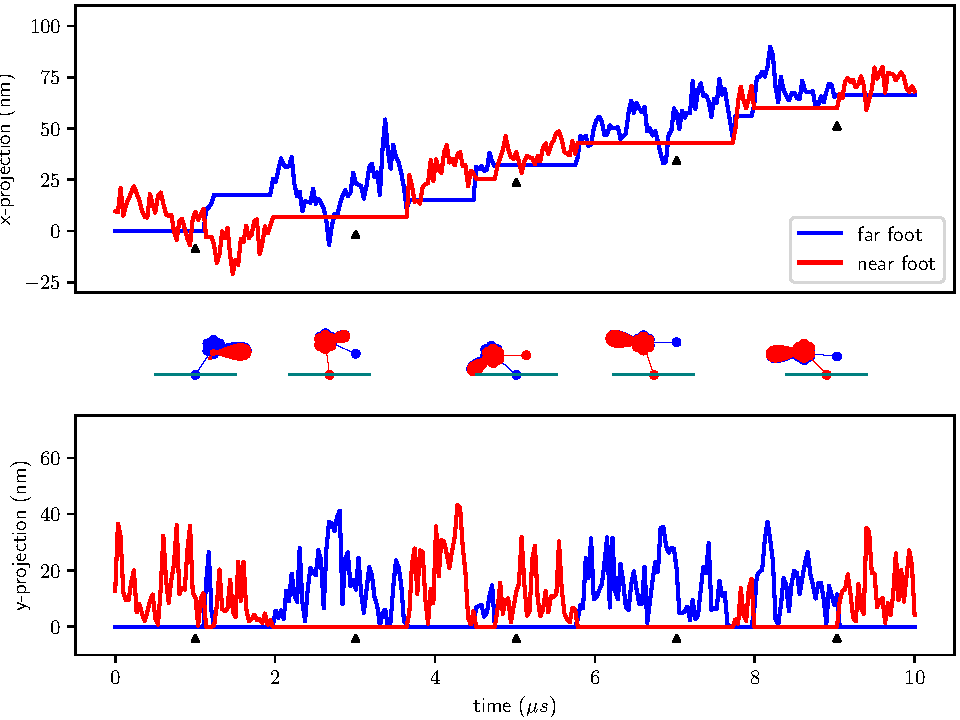
\includegraphics[width=0.65\columnwidth]{paper_trajectory_plot}
			\caption{Horizontal(x) and vertical(y) projections for the binding domain as a function of time. Between each image we show a cartoon of dynein illustrating its configuration corresponding to the black marker in each graph}
			\label{fig:trajectory}
		\end{figure}
		
		In figure \ref{fig:trajectory} we can see the horizontal and vertical projections for the dynein motor protein throughout a simulation. From this graph we can make a number of interesting conclusions. First, we can clearly see the stepping behavior: while one foot (say red) is chaotically diffusing, the other (blue) is fixed on the microtubule. Furthermore, the x-projection graph demonstrates that the motor is, on average, forward directed. Interestingly, the cartoons show that the model assumes a wide range of configurations throughout the simulation. Neither the hind-leg nor human leg shape appears to be preferred. 
		
		
		\noindent\textbf{NOTE2: Need to fix bibliography style in latex to match the physical review letters style} 


\bibliography{references}
\bibliographystyle{acm}
\end{document}
